\section{Лекция 8. Проблема выпуклой оптимизации}


\subsection{Постановка задачи}
\begin{itemize}
    \item Задача выпуклой оптимизации: $\min\{f(x): x\in X\}$.
\end{itemize}
\begin{itemize}
    \item Целевая функция $f:\mathbb{R}^n \rightarrow \mathbb{R}$ дифференцируемая и выпуклая.
\end{itemize}
\begin{itemize}
    \item Множество допустимых решений:\\
$X = \{x \in X^{(0)}: g^{(i)} (x) \leq 0 для всех i\in[m], h^{(i)} (x) = 0 для всех i\in[p]\}$
\end{itemize}
\begin{itemize}
    \item $X^{(0)}\subseteq \mathbb{R}^n$ замкнутое выпуклое множество (простой структуры).
\end{itemize}
\begin{itemize}
    \item $g^{(1)} ,\ldots,g^{(m)}:\mathbb{R}^n \rightarrow \mathbb{R}$ дифференцируемые и выпуклые функции.
\end{itemize}
\begin{itemize}
    \item  $h^{(1)} ,\ldots,h^{(p)}:\mathbb{R}^n \rightarrow \mathbb{R}$ аффинные функции.
\end{itemize}
\begin{itemize}
    \item Таким образом, $X$ замкнутое выпуклое множество.
\end{itemize}

\subsection{Радиальные и нормальные конусы}
\textbf{Определение 3.1}\\
Пусть $ X\subseteq\mathbb{R}^n$ и $x^* \in X$. Тогда радиальный конус (конус направлений) множества $X$ в точке $x^*$ -- это множество:
\begin{center}
    $K_{x^*}(X):= cone(X-\{x^*\})=\{\lambda(x-x^*)| x \in X, \lambda \geq 0\}$\\
\end{center}
\begin{center}
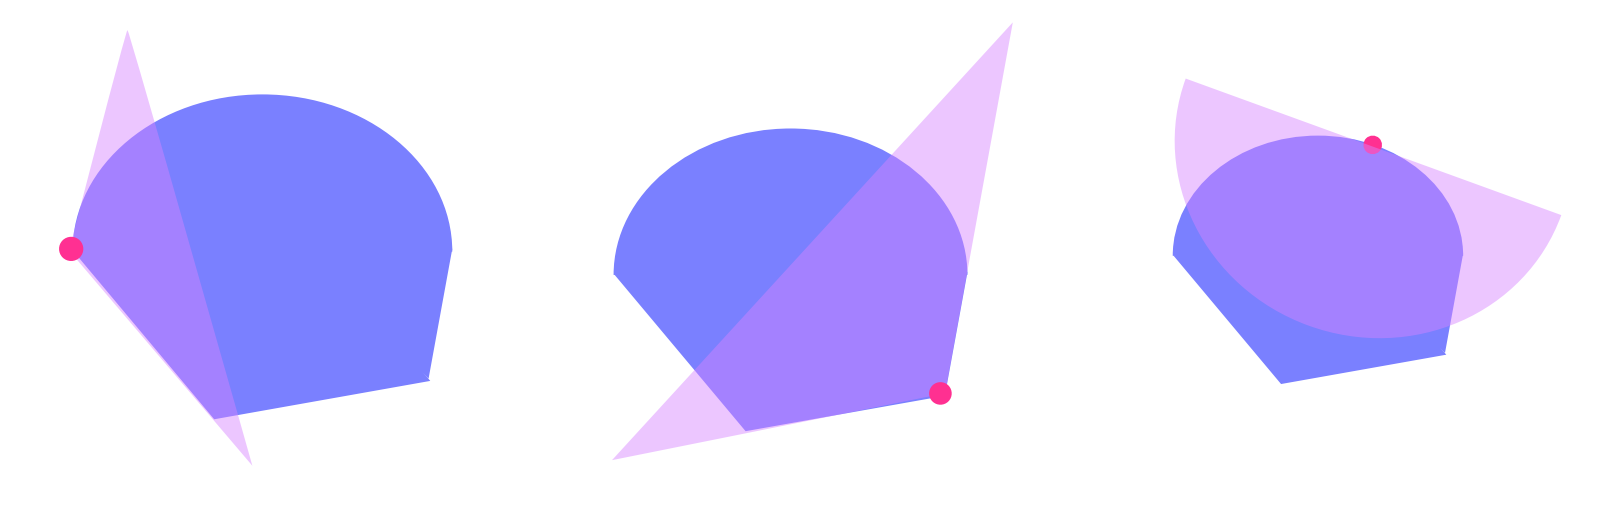
\includegraphics[scale=0.3]{radk.png}
\end{center}
\noindent\textbf{Наблюдение 3.2}\\
Если $x^*$ внутренняя точка из $X$, тогда $K_{x^*}(X)=\mathbb{R}^n$\\

\noindent\textbf{Определение 3.3}\\
Пусть $ X\subseteq\mathbb{R}^n$ и $x^* \in X$. Тогда нормальный конус множества $X$ в точке $x^*$ -- это множество: $N_{x^*}(X):= K_{x^*}(X)\circ$\\
\begin{center}
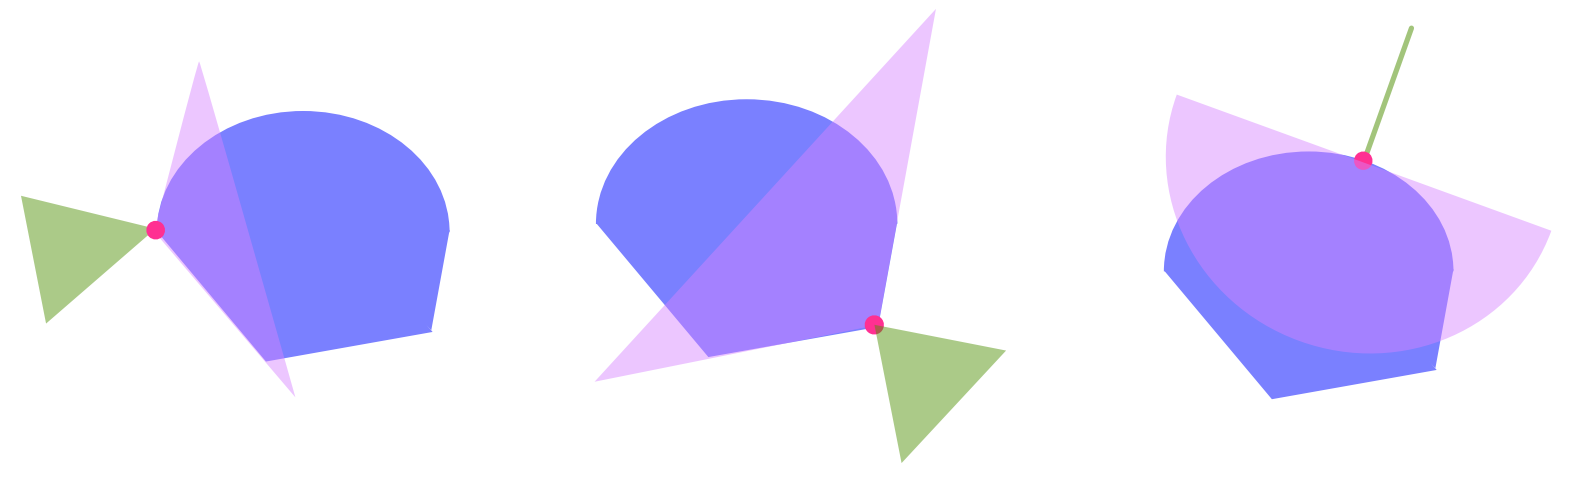
\includegraphics[scale=0.3]{normk.png}
\end{center}
\noindent\textbf{Наблюдение 3.4}\\
Если $x^*$ внутренняя точка из $X$, тогда $N_{x^*}(X)=\left\lbrace\mathbb{O}_n\right\rbrace$\\
\subsection{Радиальные и нормальные конусы для полиэдра}
Пусть $A\in\mathbb{R}^{m\times n}$, $b\in\mathbb{R}^{m}$ и $x^*\in\mathbb{R}^n$, причём $A x^*\leq b:$
\begin{equation*}
Eq_{Ax\leq b}(x^*):= \{i\in[m] | \langle A_{i,*},x^* \rangle = b_{i} \subseteq [m]\}
\end{equation*}
Радиальный конус для полиэдра $Ax \leq b$ в точке $x^*$ -- это все направления $y$, такие, что:
\begin{center}
$\exists \lambda > 0 : A(x^* + \lambda y) \leq b$\\
$A x^* + \lambda A y \leq b$\\
\end{center}
Строки $\langle A_{i,*},x^* \rangle \leq b_{i}$ задают любое направление $y$, а строки $\langle A_{i,*},x^* \rangle = b_{i}$ дают только те направления $y$, для которых $\langle A_{i,*},y \rangle \leq 0$.\\

\noindent\textbf{Замечание 3.5}\\
Пусть $x^*\in P^{\leq}(A,b) = \{x\in\mathbb{R}^n | Ax \leq b\} (A\in\mathbb{R}^{m \times n} и b\in\mathbb{R}^m)$. Тогда справедливо:
\begin{center}
    $K_{x^*}(P^{\leq}(A,b)) = \{y\in\mathbb{R}^n | \langle A_{i,*},y \rangle \leq 0 для любых i \in Eq_{Ax \leq b}(x^*)\}$\\
\end{center}
\begin{center}
    $N_{x^*}(P^{\leq}(A,b)) = ccone\{ A_{i,*} | i \in Eq_{Ax \leq b}(x^*)\}$\\
\end{center}
В частности, радиальный и нормальный конусы полиэдра -- полиэдрические конусы.\\

\subsection{Оптимизация дифференцируемой функции на выпуклом множестве.}
\textbf{Теорема 3.6}\\
Пусть $f: X \rightarrow \mathbb{R}$ дифференцируемая функция, заданная на выпуклом множестве $X\subseteq\mathbb{R}^n$.
\begin{enumerate}
    \item Если $f$ принимает в точке $x^*\in X$ локальный минимум на $X$, то $-grad_{x^*}(f)\in N_{x^*}(X)$
    \item Если $f$ выпуклая и $-grad_{x^*}(f)\in N_{x^*}(X)$, то $f(x^*)=\min\{f(x) | x \in X\}$\\
\end{enumerate}

\noindent$\blacktriangleleft$ Пусть:
\begin{enumerate}
    \item $f$ принимает в $x^*$ локальный минимум на $X$.\\
\begin{itemize}
\item Предположим  $-grad_{x^*}(f) \notin N_{x^*}(X)$.
\item Это значит: $-grad_{x^*}(f) \notin K_{x^*}(X)\circ$
\item $\Longrightarrow \exists \lambda \geq 0, x \in X: \langle -grad_{x^*}(f), \lambda (x-x^*)\rangle > 0,$
\item $\lambda (x-x^*) \in K_{x^*}(X)$
\item т.к. $(\lambda \neq 0) \Longrightarrow \langle grad_{x^*}(f),x-x^*\rangle < 0$.
\item Рассмотрим функцию $\phi: t \rightarrow f(x^* + t(x - x^*))$, тогда $\langle grad_{x^*}(f),x-x^*\rangle = \phi '(0)$
\item $\phi '(0) < 0$ $\Rightarrow$ $\exists$ достаточно малое $0<\epsilon \leq 1 : f(x^{*}+\epsilon (x-x^{*}))= \phi(\epsilon) < \phi(0) = f(x^{*})$, $x^* + \epsilon(x - x^*) \in X$
\item $X$ выпуклое множество, $x,x^{*} \in X$ и $x^{*} + \epsilon(x-x^{*})$ принадлежит окресности $x^{*}$.
\item Получили противоречие с тем, что в $x^{*}$ достигается локальный минимум.
\item Следовательно, $-grad_{x^*}(f) \in N_{x^*}(X)$.
\end{itemize}
    \item Пусть $f$ выпуклая функция и $-grad_{x^{*}}(f) \in N_{x^{*}}(X)$.\\
\begin{itemize}
\item Пусть $x \in X$ произвольная точка.
\item Для всех $t \in ]0,1]$ справедливо:
\begin{equation*}
f(x^{*} + t(x - x^{*})) = f((1 - t)x^{*} + t x) \leq (1 - t)f(x^{*}) + t f(x) = f(x^{*}) + t(f(x) - f(x^{*})) $$\\$$
\Longrightarrow \displaystyle\frac{f(x^{*} + t(x - x^{*})) - f(x^{*})}{t} \leq f(x) - f(x^{*})
\end{equation*}
\item $\displaystyle\frac{f(x^{*} + t(x - x^{*})) - f(x^{*})}{t} \displaystyle\rightarrow_{t\rightarrow 0} \phi '(0) = \langle grad_{x^{*}}(f),x - x^{*} \rangle$
\item $\langle grad_{x^{*}}(f),x - x^{*} \rangle \leq f(x) -f(x^{*})$
\end{itemize}
$\langle grad_{x^{*}}(f),x - x^{*} \rangle \geq 0$ [т.к. $x - x^{*} \in K_{x^{*}}(X)$] $\Rightarrow$ $f(x^{*}) \leq f(x)$. $\blacktriangleright$\\
\end{enumerate}

\noindent\textbf{Следствие 3.7}\\
Дифференцируемая выпуклая функция $f$ принимает свой (глобальный) минимум в точке $x^{*}$ на множестве $X$ тогда и только тогда, когда $-grad_{x^{*}}(f) \in N_{x^{*}}(X)$.\\

\noindent\textbf{Замечания к теореме 3.6 (следствию 3.7)}
\begin{enumerate}
    \item Если $x^{*} \in int(X)$, тогда $N_{x^{*}}(X) = \{\mathbb{O}\}$ и тогда в условии теоремы $grad_{x^{*}}(f) = \mathbb{O}$.
    \item Теорема 3.6/ следствие 3.7 не говорят о существовании оптимального решения.\\
Пример: $\min\mathbb{e}^x$, $x\in\mathbb{R}$ или $\min y$, при условии $y \geq 1/x, x > 0$.
\end{enumerate}

\subsection{Некоторые нормальные конусы}
\textbf{Лемма 3.8}\\
Если $K\subseteq\mathbb{R}^n$ и $x^{*} \in K$, тогда $N_{x^{*}}(K) = \{y \in K^{\circ} | \langle x^{*},y \rangle = 0\}$.\\

\noindent\textbf{Замечание 3.9}
\begin{enumerate}
    \item $x^{*} \in \mathbb{R}_{+}^{n}$ (1-й ортант), тогда $N_{x^{*}}(\mathbb{R}_{+}^{n}) = \{y\in\mathbb{R}_{-}^{n} | y_{i}=0 для всех i\in[n], x_{i}^{*}>0\}$
    \item $X^{*}\in\mathbb{S}_{+}^{k}$ (положительно определённая матрица), тогда $N_{X^{*}}(\mathbb{S}_{+}^{k}) = \{Y\in\mathbb{S}_{-}^{k} | \langle X^{*},Y \rangle = 0\}$  (скалярное произведение Фробениуса)
\end{enumerate}

\noindent\textbf{Замечание 3.10}\\
$K_{i}\subseteq\mathbb{R}^{n_{j}} (i\in[r])$ и $(x^{(1)},\ldots,x^{(r)}) \in K_{1}\times\ldots\times K_{r}$, тогда $N_{(x^{(1)},\ldots,x^{(r)})}(K_{1}\times\ldots K_{r}) = N_{x^{(1)}}(K_{1})\times\ldots\times N_{x^{(r)}}(K_{r})$

\newpage
\subsection{Условия Каруша-Куна-Таккера. Постановка задачи}
$(X_{0},(g_{(i)})_{i\in[m]},(h_{(i)})_{i\in[p]})$\\
\begin{itemize}
    \item $X_{0}\subseteq\mathbb{R}^n$ выпуклое.
\end{itemize}
\begin{itemize}
    \item $g_{i}:\mathbb{R}^n\rightarrow\mathbb{R}$ выпуклые и дифференцируемые $(i\in[m])$
\end{itemize}
\begin{itemize}
    \item $h_{i}:\mathbb{R}^n\rightarrow\mathbb{R}$ аффинные $(i\in[p])$\\
\end{itemize}
Множество допустимых решений:\\
$X = {x \in X_{0} | g^{(i)}(x) \leq 0 для всех i\in[m], h^{(i)}(x) = 0 для всех i\in[p]}$\\
Иная запись
\begin{equation*}
X = X_{0}\cap\bigcap_{i\in[m]}G_{i}\cap\bigcap_{i\in[p]}H_{i}
\end{equation*}
где $G_{i}:=g_{i}^{-1}(\mathbb{R}_{-})$ и $H_{i}:=h_{i}^{-1}({0})\subseteq\mathbb{R}^n$.
\subsection{Нормальный конус для регулярной тройки}
\textbf{Лемма 3.11}\\
Если $(X_{0},(g_{(i)})_{i\in[m]},(h_{(i)})_{i\in[p]})$ регулярная, тогда:
\begin{center}
    $N_{x*}(X) = N_{x*}(X_{0}) + \sum_{i\in[m]}{N_{x*}(G_{i})} + \sum_{i\in[p]}{N_{x*}(H_{i})}$.\\
\end{center}
$(X_{0},(g_{(i)})_{i\in[m]},(h_{(i)})_{i\in[p]})$ регулярная если:
\begin{enumerate}
    \item Множество $X_{0}$ -- полиэдр и функции $g_{1},\ldots,g_{m}$ аффинные\\ или
    \item Множество $X\bigcap int(X_{0})$ не пусто и функции $g_{1},\ldots,g_{m}$ аффинные\\ или
    \item Существует точка $x^{(s)} \in X$ $(x^{(s)} \in int(X_{0}), если p \neq 0)$ такая, что $g_{i}(x^{(s)}) < 0$ для всех $i\in[m]$ (условие Слейтера)\\
\end{enumerate}
\noindent$\blacktriangleleft$ (Лемма 3.11)\\
$N_{x*}(x) = (K_{x*}(x))^{\circ} = (K_{x*}(X_{0})\cap\bigcap_{i=1}^{m} K_{x*}(G_{i})\cap\bigcap_{i=1}^{p} K_{x*}(H_{i}))^{\circ}$
\begin{enumerate}
\item
\begin{itemize}
    \item Все радиальные конусы полиэдрические, из следствия 2.47:\\
    $\Rightarrow (K_{x*}(X_{0})\bigcap\bigcap_{i=1}^{m} K_{x*}(G_{i})\bigcap\bigcap_{i=1}^{p} K_{x*}(H_{i}))^{\circ} = N_{x*}(X)$
     \item $N_{x*}(X) = N_{x*}(X_{0}) + \sum_{i\in[m]}{N_{x*}(G_{i})} + \sum_{i\in[p]}{N_{x*}(H_{i})}$
\end{itemize}
\item
    \begin{itemize}
    \item $K_{1} := \bigcap_{i=1}^{m} K_{x*}(G_{i})\cap\bigcap_{i=1}^{p} K_{x*}(H_{i})$
    \item $K_{2} := K_{x*}(X_{0})$ т.к. $X \bigcap int(X_{0})$ не пусто, то $K_{1} \bigcap int(K_{2}) \neq \varnothing$
    \item Из теоремы 2.39 $\Rightarrow (K_{1} \bigcap K_{2})^{\circ} = K_{1}^{\circ} + K_{2}^{\circ}$
    \item По следствию 2.47 $\Rightarrow (K_{x*}(X_{0})\cap\bigcap_{i=1}^{m} K_{x*}(G_{i})\cap\bigcap_{i=1}^{p} K_{x*}(H_{i}))^{\circ} = N_{x*}(X)$
    \item $N_{x*}(X) = N_{x*}(X_{0}) + \sum_{i\in[m]}{N_{x*}(G_{i})} + \sum_{i\in[p]}{N_{x*}(H_{i})}$
    \end{itemize}
    \item
    \begin{itemize}
    \item $p=0$:
    	\begin{itemize}
    \item $K_{1} := K_{x*}(X_{0})$, $K_{i+1} := K_{x*}(G_{i})$ $i\in[m]$
    \item $\Rightarrow_{x^{(s)}}$ $K_{1}\bigcap\bigcap_{i=2}^{m+1}int(K_{i})\neq\varnothing$
    \item $\Rightarrow_{теорема 2.39}$ $(K_{x*}(X_{0})\bigcap\bigcap_{i=1}^{m}K_{x*}(G_{i}))^{\circ} = N_{x*}(X_{0}) + 			\sum_{i\in[m]}{N_{x*}(G_{i})}$
		\end{itemize}
	\item $p>0$:
		\begin{itemize}
			\item $K_{1} := K_{x*}(H_{i})$, $K_{2} := K_{x*}(X_{0})$, $K_{i+2} := K_{x*}(G_{i})$ $i\in[m]$
		\item $\Rightarrow_{x^{(s)}}$ $K_{1}\bigcap\bigcap_{i=2}^{m+2}int(K_{i})\neq\varnothing$
		\item По теореме 2.39, следствию 2.47:\\
		$(K_{x*}(X_{0})\bigcap\bigcap_{i=1}^{m} K_{x*}(G_{i})\bigcap\bigcap_{i=1}^{p} K_{x*}(H_{i}))^{\circ} = N_{x*}(X)$
		\item $N_{x*}(X) = N_{x*}(X_{0}) + \sum_{i\in[m]}{N_{x*}(G_{i})} + \sum_{i\in[p]}{N_{x*}(H_{i})}$
		\end{itemize}
    \end{itemize}
	 $\blacktriangleright$
\end{enumerate}
